\documentclass[xcolor={svgnames},aspectratio=169]{beamer}
\usetheme[progressbar=frametitle]{metropolis}

\usepackage[utf8]{inputenc}
\usepackage{graphicx}
\usepackage{courier}
\usepackage{listings}
\usepackage{mathpartir}

\usepackage[autostyle]{csquotes}
\usepackage[
    backend=biber,
    style=authoryear-icomp,
    sortlocale=de_DE,
    natbib=true,
    url=false, 
    doi=false,
    eprint=false
]{biblatex}
\addbibresource{biblio.bib}

\usepackage[svgnames]{xcolor}
\xdefinecolor{darkgreen}{named}{DarkGreen}

\lstdefinelanguage{lustre}{%
   columns=fullflexible,%
   basicstyle=\tt\footnotesize,
   % keywordstyle=\bfseries,
   commentstyle=\slshape,%
   keywords={%
     node,var,let,tel,returns,
     when,merge
   },%
   keywordstyle={\color{darkgreen}\sffamily},%
   morekeywords=[2]{%
     int, real, bool,
   },%
   keywordstyle=[2]{\color{blue}\ttfamily},%
   classoffset=2,%
   morekeywords=[3]{%
     storage, parameter, code %
   },%
   morekeywords=[3]{
     True,False
   },
   keywordstyle=[3]{\color{purple}},%
   sensitive,%
   morestring=[d]",%"
}[keywords,comments,strings]%

\lstMakeShortInline[language=albert]?

\lstset{language=lustre}

\title{Un compilateur pour le langage Minilucy}
\author{Basile Pesin}

\begin{document}

\maketitle

\section{Organisation du projet}

\begin{frame}{Choix techniques}
  \begin{itemize}
    \item Ecrit en OCaml + Menhir pour le parsing
    \item 3700loc (avec un peu de répétition dans les AST successifs)
    \item Syntaxe très proche du Lustre ``traditionnel''
  \end{itemize}
\end{frame}

\begin{frame}{Chaine de compilation}
  \begin{center}
    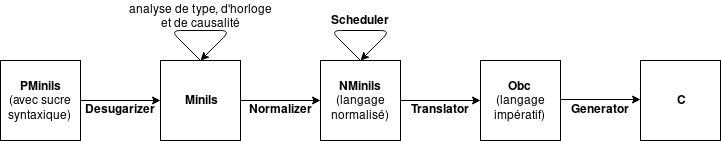
\includegraphics[width=.8\paperwidth]{assets/chain.png}
    Proche de l'organisation décrite dans~\citep{Biernacki08}
  \end{center}
\end{frame}

\section{Affinage du typage d'horloge}

\begin{frame}{Horloges implicites}
  Dans l'article, pas de sous-typage (sous-échantillonage implicite) : on doit mettre des \lstinline{when} partout. Dans les faits on peut pour plus de clarté sous-échantillonner les constantes (au moins) implicitement:

$$\inferrule*
    { }
    { H \vdash v : ck }
$$

Des règles de sous-échantillonage implicites plus large seraient plus difficile à mettre en place
\end{frame}

\begin{frame}{Polymorphisme d'horloge}
  Dans l'article, l'appel à un noeud interne doit se faire avec des paramètres sur la même horloge:
$$\inferrule*
    { H \vdash a_1 : ck \ldots H \vdash a_n : ck & H \vdash a : ck }
    { H \vdash v : f(a_1, \ldots, a_n)\:every\:a : ck \times \ldots \times ck }
$$
Un peu limitant. Polymorphisme d'horloge facile (en utilisant l'horloge du \lstinline{every} comme base du noeud interne.
\end{frame}

\begin{frame}[fragile]{Polymorphisme d'horloge - exemple}
\begin{lstlisting}
node test_op(b : bool) returns (z : int when True(b));
let
  z = 3 when True(b);
  // Ou z = 3; (sous-echantillonage implicite)
tel;

node test_app(c1 : bool; b1 : bool when True(c1))
returns (z : int when True(c1) when True(b1));
let
  z = test_op(b1);
tel;
\end{lstlisting}
\end{frame}

\section{Automates}

\begin{frame}[fragile]{Automates à états - exemple}
  Inspiré de~\citep{Colaco05}
\begin{lstlisting}
node auto_simpl() returns (x : int);
let
  automaton
  | INC ->
    let u : int = (1 + pre u) in
    x = 0 fby x + u;
    until x > 5 then DEC;
  | DEC ->
    let u : int = 2 in
    x = 0 fby x - u;
    until x < -10 then INC;
  end;
tel;
\end{lstlisting}
\end{frame}

\begin{frame}[fragile]{Automates à états - compilation}
  \lstset{basicstyle=\tt\scriptsize}
  Génère des horloges d'état avec constructeurs $\equiv$ branches:

  \lstinline{type _ty_auto_state3 = DEC + INC;}

  Les expressions sont sous échantillonnées par l'horloge d'état:

  \lstinline{x = merge auto_state3 (DEC -> ...) (INC -> ...);}

  L'état est modifié par les \lstinline{until}:

  \begin{lstlisting}
auto_state3 = (INC fby (merge auto_state3
  (DEC -> (if (x < -10) then INC else DEC) when DEC(auto_state3))
  (INC -> (if (x > 5) then DEC else INC) when INC(auto_state3))));
  \end{lstlisting}
\end{frame}

\begin{frame}[fragile]{Automates à états - reset}
  \lstset{basicstyle=\tt\scriptsize}
  Un flot de reset par branche.
  Dans l'exemple
  \begin{lstlisting}
auto_state3INC_reset = merge auto_state3
                             (DEC -> true when DEC(auto_state3))
                             (INC -> false when INC(auto_state3))
  \end{lstlisting}
  Permet de contrôler les reset de \lstinline{fby} et \lstinline{every}

  Dans l'exemple l'expression de \lstinline{x} pour la branche \lstinline{INC} devient:
  \begin{lstlisting}
    if (pre (auto_state3INC_reset when INC(auto_state3)))
    then 0
    else (0 fby ((x when INC(auto_state3)) + let_u1)))
  \end{lstlisting}
  Avec \lstinline{let_u1} une variable utilisée pour le \lstinline{let} binding local de \lstinline{u}
\end{frame}

\section{Interpréteur et vérification}

\begin{frame}{Un interpréteur naïf pour le langage Lustre}
  Une expression génère une fonction de transition:
  $(Etat \times Entrées) \rightarrow (Etat \times Sorties)$

  L'état d'un noeud contient
  \begin{itemize}
  \item les flots depuis le début de l'exécution (coûteux en mémoire)
  \item l'état des noeuds internes
  \end{itemize}

  Ordonnancement ``dynamique'' : pendant l'exécution on va calculer ce dont en a besoin (cycles détectés)
\end{frame}

\begin{frame}{Interpréteur étendu aux automates}
  On ajoute les automates à notre interpréteur !

  Un peu plus complexe : il faut gérer les états, flots de reset... Mais pas tellement (70 loc de plus pour les automates)
\end{frame}

\begin{frame}{Vérification dynamique}
  \begin{center}
    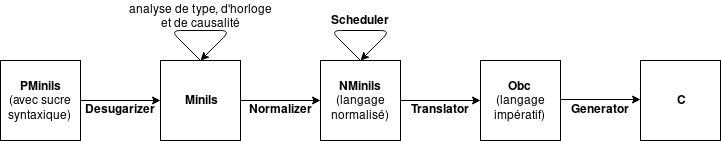
\includegraphics[width=.8\paperwidth]{assets/chain.png}
  \end{center}
  On vérifie:
  \begin{itemize}
    \item \textbf{desugarizer}: interprète à automate = interprète noyau
    \item \textbf{normalisation}: inlining des équations normalisées = équations
    \item \textbf{ordonnancement}: même ensemble d'équations triées
    \item \textbf{traduction}: plus difficile (langages très différents), donc on vérifie seulement que toutes les sorties sont bien déclarées (assez faible). Un troisième interpréteur ?
    \item \textbf{generation}: pas très intéressant à vérifier
  \end{itemize}
\end{frame}

\section{AVR-Lustre}

\begin{frame}{Lustre embarqué, pour pas très cher}
  Constatations:
  \begin{itemize}
    \item Lustre est souvent utilisé dans l'embarqué critique
    \item Les microcontrôleurs peuvent être programmés en C
    \item Notre compilateur compile vers C !
  \end{itemize}

  On a juste besoin d'un runtime pour les IOs (on utilise celle d'OMicroB~\citep{VVC18})
\end{frame}

\begin{frame}{Cible choisie}
  \textbf{Arduino Uno}: très utilisée par les hobbyiste + prototypage
  \begin{columns}[T]
    \begin{column}{.65\textwidth}
      \begin{itemize}
      \item Architecture AVR (AtMega328P)
      \item 16ko de mémoire Flash
      \item 2ko de mémoire SRAM
      \item 14 broches d'IO numériques, dont 6 avec PWM (sortie pseudo-analogique)
      \item 6 broches d'entrées analogiques
      \end{itemize}
    \end{column}
    \begin{column}{.46\textwidth}
      \vspace{0.5cm}
      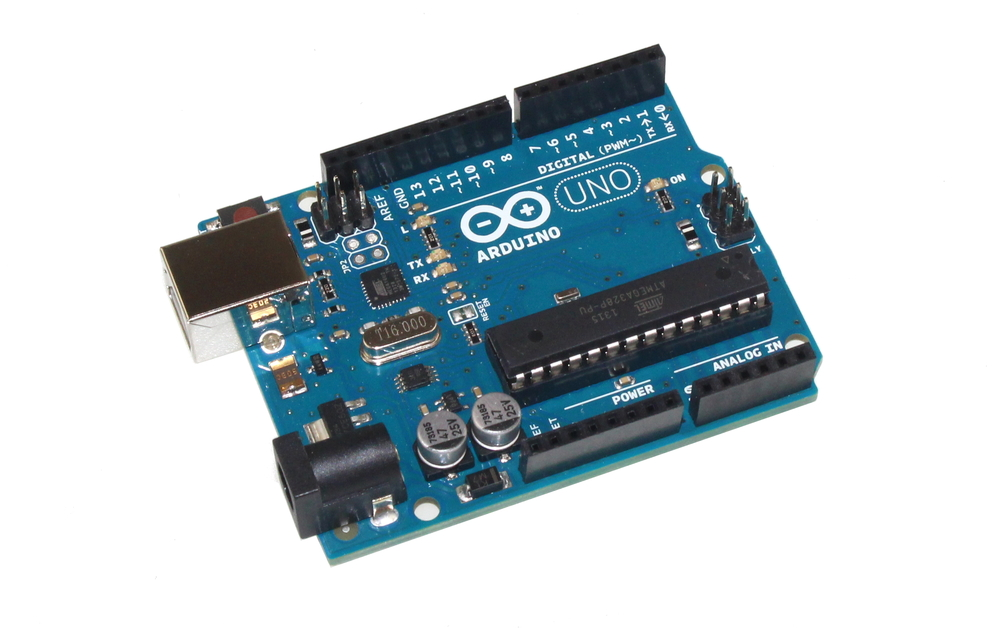
\includegraphics[width=.35\paperwidth]{assets/uno.jpg}
    \end{column}
  \end{columns}
\end{frame}

\begin{frame}[fragile]{AVR-Lustre, utilisation}
\lstset{basicstyle=\tt\scriptsize}
  \begin{columns}[T]
    \begin{column}{.5\textwidth}
      Code Lustre:
      \begin{lstlisting}
node main(b1 : bool; b2 : bool;
          x : int)
returns (b : bool; y : int);
let
  b = b1 or b2;
  y = 2 * x;
tel;
      \end{lstlisting}
      Définition des entrées-sorties:
      \lstset{language=[ANSI]C,basicstyle=\tt\scriptsize}

      \begin{lstlisting}
#define CLOCK_PERIOD 10

void io_init() {
  avr_pin_mode(PIN4, INPUT);
  avr_pin_mode(PIN5, INPUT);
  avr_pin_mode(PIN7, OUTPUT);

  avr_pin_mode(PINA1, INPUT);
  avr_pin_mode(PIN3, OUTPUT);
}
      \end{lstlisting}
    \end{column}
    \begin{column}{.5\textwidth}
      \lstset{language=[ANSI]C,basicstyle=\tt\scriptsize}
      \begin{lstlisting}
int io_read_b1() {
  return avr_digital_read(PIN4);
}

int io_read_b2() {
  return avr_digital_read(PIN5);
}

int io_read_x() {
  return avr_analog_read(PINA1);
}

void io_write_b(int b) {
  avr_digital_write(PIN7, b);
}

void io_write_y(int y) {
  avr_analog_write(PIN3, y);
}
      \end{lstlisting}
    \end{column}
  \end{columns}
\end{frame}

\section{Demo !}

\begin{frame}
  \printbibliography
\end{frame}

\end{document}
